Para crear la tarea pedida, creamos un nuevo método en el archivo \texttt{task.cpp} llamado \texttt{TaskConsola}. El código que implementa la solución es sumamente simple.

La tarea itera sobre la cantidad de llamadas bloqueantes que el usuario pasó por parámetro, generando por cada iteración un número pseudoaleatorio, \texttt{nro\_random}, y realizando la respectiva llamada de \emph{I/O} (cuya duración es \texttt{nro\_random}).

Notar que para aumentar el grado de aleatoriedad inicializamos el valor de la semilla a partir del tiempo del sistema, en lugar de un valor fijo, cada vez que se llama a \texttt{TaskConsola}.

Es importante que, aunque no se vea en nuestro código, antes de bloquearse la tarea tiene que gastar un ciclo en el CPU, justamente para poder hacer la solicitud de \emph{I/O}.

La figura \ref{fig:ej1} nos ayuda a entender mejor el funcionamiento de este tipo de tarea: los procesos 2 y 3 entran juntos en tiempo 0, el 0 y 1 en tiempo 5. Cada par corre en paralelo gracias a que hay dos procesadores, lo que facilita la comparación. El objetivo del primer par es ilustrar el caso en que la duración de las llamadas bloqueantes está prefijada: ambos procesos hacen dos llamadas de \emph{I/O} cuya duración es exactamente 4 (para lograr esto hacemos que \texttt{bmin=bmax=4}). Por otra parte, los procesos 0 y 1, aunque reciben los mismos parámetros cada uno, muestran comportamientos distintos debido a que el rango de duración de cada bloqueo es de longitud mayor a 0. 

Puede verse también que el tiempo que cada proceso pasa en el CPU antes de bloquearse es de exactamente un ciclo, que es lo que tarda en hacer la solicitud de \emph{I/O}. En el último ciclo de cada proceso se hace el \texttt{exit}. Ambas cosas no dependen directamente de nuestro código, sino de las implementaciones de \texttt{uso\_IO} y el simulador. 


\begin{figure}[H]
  \centering
  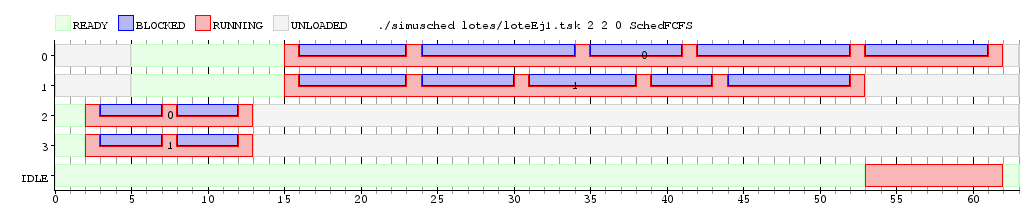
\includegraphics[width=\textwidth]{img/imgEj1-1.png}
  \caption{}
  \label{fig:ej1}
\end{figure}